% =============================================================================
\section{Squeezing near a Feshbach resonance}
% =============================================================================

In the previous section we have discussed an experiment where squeezing was achieved with component-dependent potentials which helped to reduce the inter-component interaction.
The same effect can be achieved differently --- by manipulating the external magnetic field near a Feshbach resonance for a chosen pair of hyperfine states.
This allows one to vary the interaction in a wide range with a relative ease.
The downside of this approach is the significant increase of the inter-component nonlinear loss rate accompanying the change in the interaction strength.
This results in the destruction of the squeezing as the two components interfere with each other.

The truncated Wigner approach allows us to investigate the combined effect of reduced interaction strength and increased losses.
In this section we will consider a hypothetical interferometry experiment with two hyperfine states of \Rb{} and demonstrate how with the help of the Wigner method we can pick the optimal value of the magnetic field that would lead to the maximum squeezing.

The experiment follows the general scheme used in this and the previous chapters.
We start from a \abbrev{bec} of $N = 55000$ \Rb{} atoms in the hyperfine state ${\ket{F=1,\, m_F=+1}}$ in a cigar-shaped trap with the frequencies $f_x = f_y = 97.0\un{Hz}$ and $f_z = 11.69\un{Hz}$.
The first $\pi/2$-pulse creates an equal superposition of two states, ${\ket{F=1,\, m_F=+1}}$ and ${\ket{F=2,\, m_F=-1}}$.
The external magnetic field of strength $B \approx B_0$ is applied, where $B_0 = 9.1\un{G}$ corresponds to the Feshbach resonance for the two hyperfine used~\cite{Kaufman2009}.
We then investigate the dependence of the time dependence of the maximum degree of spin squeezing.
Intra-species interaction strengths do not depend on the external magnetic field, and are taken to be $a_{11} = 100.4\,r_B$ and $a_{22} = 95.44\,r_B$.

The dependence of the inter-species interaction and loss rate can be described with a single equation for the complex scattering length~\cite{Kaufman2009}
\begin{eqn}
    a(B)
    = a_{\mathrm{bg}} \left(
        1 - \frac{\Delta B}{(B - B_0) - i \gamma_B / 2}
        \right),
\end{eqn}
where $a_{\mathrm{bg}}$ is the background scattering length, $\tilde{B}$ is the resonance width, and $\gamma_B$ is the decay width.
For a given $B$ the real part of this value acts as the $s$-wave scattering length $a_{12}$ in~\eqnref{bec-noise:system:g}:
\begin{eqn}
\label{eqn:bec-squeezing:feshbach:g}
    g_{12}(B)
    = \frac{4 \pi \hbar^2 \Real a(B)}{m}
    = \frac{4 \pi \hbar^2 a_{\mathrm{bg}}}{m} \left(
        1 - \frac{\Delta B (B - B_0)}{(B - B_0)^2 + \gamma_B^2 / 4}
    \right),
\end{eqn}
and the imaginary part can be connected to the loss rate by substituting it into~\eqnref{bec-noise:system:g} as well and comparing the resulting expression with the corresponding loss term in~\eqnref{bec-noise:mean-field:cgpes-simplified}:
\begin{eqn}
\label{eqn:bec-squeezing:feshbach:gamma}
    \gamma_{12}(B)
    = -\frac{8 \pi \hbar \Imag a(B)}{m}
    = \frac{4 \pi \hbar a_{\mathrm{bg}} \Delta B \gamma_B}{(B - B_0)^2 + \gamma_B^2 / 4}.
\end{eqn}

\begin{figure}
    \centerline{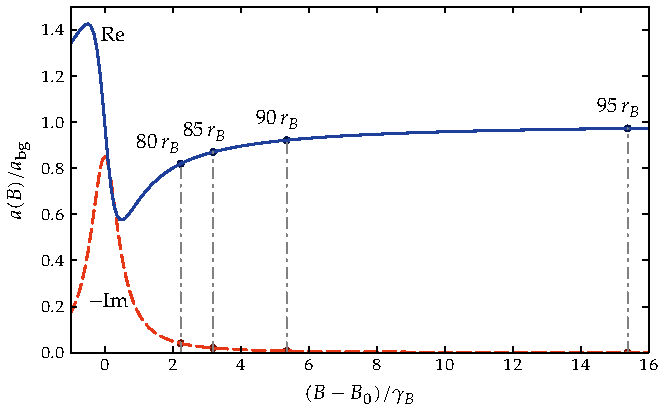
\includegraphics{figures_generated/bec_squeezing/feshbach_scattering.pdf}}

    \caption{
    Real (blue solid line) and imaginary (red dashed line, negated value is plotted for compactness) parts of the complex scattering length near the Feshbach resonance at $B_0 = 9.1047\un{G}$.
    Four pairs of points show the distances from the resonance chosen for the simulation.
    }

    \label{fig:bec-squeezing:feshbach:scattering}
\end{figure}

For the hyperfine states we use the reported resonance parameters are $B_0 = 9.1047\un{G}$, $\Delta B = 2\times10^{-3}\un{G}$, $\gamma_B = 4.7\times10^{-3}\un{G}$, and $a_{\mathrm{bg}} = 97.7\,r_B$.
The behavior of the real and the imaginary part of $a(B)$ near the resonance is shown in~\figref{bec-squeezing:feshbach:scattering}.
From the equations above, as well as from the figure, it is obvious that the minimum inter-species scattering length is achieved when $B - B_0 = 0.5 \gamma_B$.
Unfortunately, this value also corresponds to the relatively large value of the imaginary part, and, correspondingly, the loss rate.
Therefore, we will pick the values of $B$ further from the resonance, as displayed in the figure, where the interaction is somewhat stronger, but the loss rate is much smaller.
The equations~\eqnref{bec-squeezing:feshbach:g} and~\eqnref{bec-squeezing:feshbach:gamma} give us the following values for the simulation:
\begin{eqn}
    B - B_0 & = 2.24 \gamma_B, \quad
        a_{12} = 80.0\,r_B, \quad \gamma_{12} = 3.85\times10^{-12}\un{cm^3/s},\\
    B - B_0 & = 3.20 \gamma_B, \quad
        a_{12} = 85.0\,r_B, \quad \gamma_{12} = 1.93\times10^{-12}\un{cm^3/s},\\
    B - B_0 & = 5.35 \gamma_B, \quad
        a_{12} = 90.0\,r_B, \quad \gamma_{12} = 7.00\times10^{-13}\un{cm^3/s},\\
    B - B_0 & = 15.4 \gamma_B, \quad
        a_{12} = 95.0\,r_B, \quad \gamma_{12} = 8.53\times10^{-14}\un{cm^3/s}.
\end{eqn}

\begin{figure}
    \centerline{%
    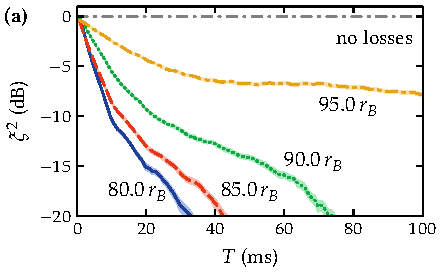
\includegraphics{figures_generated/bec_squeezing/feshbach_squeezing_no_losses.pdf}%
    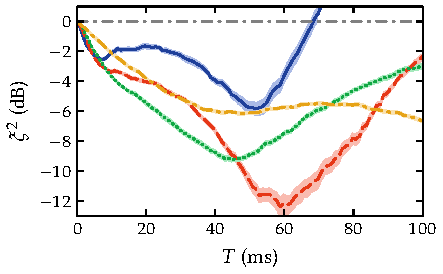
\includegraphics{figures_generated/bec_squeezing/feshbach_squeezing.pdf}}

    \caption{
    Truncated Wigner simulations of the squeezing in the vicinity of the $B_0 = 9.1047\un{G}$ Feshbach resonance in \Rb{} with different values of the external magnetic field, with \textbf{(a)}~losses turned off, and \textbf{(b)}~1--2 losses turned on.
    Results corresponding to the scattering lengths $a_{12}=80.0\,r_B$ (blue solid line), $a_{12}=85.0\,r_B$ (red dashed line), $a_{12}=90.0\,r_B$ (green dotted line), and $a_{12}=95.0\,r_B$ (yellow dash-dotted line) are plotted.
    The same-colored bands show the estimated sampling error.}

    \label{fig:bec-squeezing:feshbach:squeezing}
\end{figure}

First, we perform the simulations with $\gamma_{12}$ set to zero in order to test the squeezing in ideal conditions.
As expected, the lower $a_{12}$ is, the stronger squeezing is reachable, as shown in~\figref{bec-squeezing:feshbach:squeezing},~(a).

With the inclusion of the $1-2$ losses the picture is different.
Feshbach tuning to $a_{12} = 85.0\,r_B$ ensures the best squeezing of the four variants ($-12\un{dB}$ at $60\un{ms}$), whereas long lasting squeezing is predicted for the variant with $a_{12} = 95.0\,r_B$ (\figref{bec-squeezing:feshbach:squeezing},~(b)).
In practice, it is possible to run the simulation for more different values of $B$, thus finding the ideal balance between the interaction strength and the loss rate which produces the maximum squeezing.
